\documentclass{beamer}

\usepackage[francais]{babel}
\usepackage[utf8]{inputenc}
\usepackage[T1]{fontenc}
\usepackage{graphicx}
\usepackage{graphics}
\usepackage{color}
\usepackage{textcomp}
\usepackage{pifont}
\usepackage[normalem]{ulem}
\usepackage{times}
\usepackage{hyperref}
\usepackage{verbatim}
\usepackage{amsmath}
\usepackage{amsthm}
\usepackage{amsfonts}
\usepackage[mathscr]{euscript}
\usepackage{pgfpages}
\usepackage{listings}
\usepackage{subfigure}
\usepackage{algorithm}
\usepackage[noend]{algorithmic}
\usepackage{pdftricks}
\usepackage{mathrsfs}
\usepackage{array}
\usepackage{fancybox}
% \usepackage{columns}
\usepackage{multirow}
\usepackage{url}
\usepackage{tikz}
\usepackage{colortbl}
%\usepackage{cite} %DO NOT FUCKING USE CITE ON BEAMER !!! LOST 30 GODDAM' MINUTES ON THIS SHIT !!!
\usepackage{mathabx}
\usepackage{amssymb}
\usepackage{eurosym}
\usepackage{wasysym} % ch0

\let\texteuro\euro

\hypersetup{colorlinks,%
            citecolor=black,%
            filecolor=black,%
            linkcolor=black,%
            urlcolor=blue}

%\addtolength{\parskip}{10pt}

\usetikzlibrary{calc}

\mode<presentation>
\setbeamertemplate{footline}[frame number]
\setbeamercovered{transparent}
\usetheme[navigation]{ESI}

%lst
\definecolor{comment-green}{RGB}{0,166,80}
\lstset{language=C++,
  keywordstyle=\lst@ifdisplaystyle\bf\fi\color{blue!60},
  commentstyle=\color{comment-green},
  stringstyle=\color{red},
  basicstyle=\lst@ifdisplaystyle\tiny\else\tt\fi,
  morekeywords={
    constexpr,concept,decltype,nullptr,nullptr_t,noexcept,final,override},
  frame=single,
  xleftmargin=0.5cm,
  numbers=left,
  tabsize=2}

%title
\subtitle{Langage \texttt{C} / \cpp}
\author{R. Absil}
\date{\today}

%styles
\theoremstyle{definition}
\newtheorem{thm}{Théorème}
\newtheorem{conj}[thm]{Conjecture}
\newtheorem{deff}[thm]{Définition}
\newtheorem{prop}[thm]{Propriété}
\newtheorem{lem}[thm]{Lemme}
\newtheorem*{lem*}{Lemme}
\newtheorem{cor}[thm]{Corollaire}
%\newtheorem{example}{Exemple}
\newtheorem{remark}{Remarque}
\newtheorem{exo}{Exercice}

%typeset
\newcommand{\ie}{{\emph{i.e., }}}
\newcommand{\eg}{{\emph{e.g., }}}
\newcommand{\etal}{{\emph{et al.}}}
\newcommand{\rrceil}{\unichar{"2308}}
\newcommand{\sloand}[2]{\footnote{N. J. A. Sloane - OEIS Foundation - \texttt{www.oeis.org}, Sequence #1 - #2.}}

%math
\newcommand{\IN}{{\mathbb N}}
\newcommand{\IQ}{{\mathbb Q}}
\newcommand{\IR}{{\mathbb R}}
\newcommand{\IZ}{{\mathbb Z}}
\newcommand{\IP}{{\mathbb P}}
\newcommand{\IC}{{\mathbb C}}
\newcommand{\bigo}{{\mathcal{O}}}
\renewcommand{\mod}{\bmod}
\newcommand{\ssi}{\Leftrightarrow}
\newcommand{\then}{\Rightarrow}
\newcommand{\fle}[1]{\stackrel{#1}{\longrightarrow}}
\newcommand{\suchthat}{~\big|~}
\newcommand{\floor}[1]{\left\lfloor #1 \right\rfloor}
\newcommand{\ceil}[1]{\left\lceil #1 \right\rceil}
\DeclareMathOperator*{\argmin}{argmin}
\DeclareMathOperator*{\argmax}{argmax}

%tikz
\tikzstyle{_vertex}=[fill=white, circle,minimum size=12pt,inner sep=1pt]
\tikzstyle{_blackv}=[fill=black, circle,minimum size=8pt,inner sep=1pt]
\tikzstyle{_dot}=[fill=black, circle, minimum size = 1mm, inner sep=0pt]
\tikzstyle{_bigvertex}=[fill=white, circle,minimum size=21pt,inner sep=1pt]
\tikzstyle{_arc}=[->, >=stealth]
\tikzstyle{_boldarc}=[->, >=stealth, line width=2pt]

\newcommand{\cpp}{\texttt{C++}}
\newcommand{\java}{\texttt{Java}}


\title{Ch. 13 - Templates}

\begin{document}
\begin{frame}
  \titlepage
\end{frame}

\begin{frame}
  \frametitle{Table des matières}
  \footnotesize \tableofcontents[pausesections,pausesubsections]
\end{frame}


\section{Généralités}

\begin{frame}
\frametitle{Overview}
\begin{itemize}[<+->]
\item \emph{Introduction} au mécanisme de templates en \cpp
	\begin{itemize}
	\item Livres complets existants
	\end{itemize}
\item Très efficace
	\begin{itemize}
	\item Génération à la compilation
	\item Liaison statique des liens
	\end{itemize}
\item Permet
	\begin{itemize}
	\item de la programmation modulaire
	\item d'émuler des relations d'héritage
	\item d'émuler le polymorphisme en « compile-time »
	\item d'éviter des conversions implicites
	\end{itemize}
\item Mécanisme très différent des generics en \java
\end{itemize}
\end{frame}

\begin{frame}
\frametitle{Syntaxe}
\begin{itemize}[<+->]
\item \lstinline|template<liste params> prototype|
\item Déclare le prototype
	\begin{enumerate}
	\item d'une classe
	\item d'un membre de classe
	\item d'une fonction
	\item d'une variable
	\end{enumerate}
\item La liste des paramètres est une liste non-vide de « types » 
\end{itemize}
\end{frame}

\begin{frame}[containsverbatim]
\frametitle{Exemples}
\begin{lstlisting}
template<class T> class A {};

A<int> a;
\end{lstlisting}

\begin{lstlisting}
class B
{
	template<class T> void brol(T t);
};

B b;
b.brol(2);
\end{lstlisting}

\begin{lstlisting}
template<int N> class C {};

C<5> a;
\end{lstlisting}

\begin{lstlisting}
template<class T> T gcd(T a, T b) {...};

int a = gcd(24, 36);
\end{lstlisting}

\begin{lstlisting}
template<class T = double> constexpr T PI = T(atan(1) * 4);

double area = PI<> * r * r;
\end{lstlisting}
\end{frame}

\begin{frame}
\frametitle{Implémentation (1/2)}
\begin{block}<+->{Règle}
	\begin{itemize}
	\item Le code « concret » d'un template est généré (et compilé) à la compilation, si besoin est.
	\end{itemize}
\end{block}
\begin{exampleblock}<+->{Avantages}
	\begin{itemize}[<+->]
	\item Très efficace
	\item La taille d'un \texttt{T} est connue à la compilation
		\begin{itemize}
		\item son type « véritable » aussi
		\end{itemize}
	\item Résolution statique des liens
	\end{itemize}
\end{exampleblock}
\end{frame}

\begin{frame}
\frametitle{Implémentation (2/2)}
\begin{alertblock}<+->{Inconvénients}
	\begin{itemize}[<+->]
	\item Peut cacher des bugs
		\begin{itemize}
		\item Des bugs compilatoires ou sémantiques peuvent apparaître pour certaines spécialisations et pas d'autres
		\item Messages d'erreurs de compilation parfois obscurs
		\item Grossit la taille de l'exécutable
			\begin{itemize}
			\item Grossit la taille du segment de code
			\end{itemize}
		\item L'implémentation des prototypes se fait au sein du même fichier
			\begin{itemize}
			\item Force l'open source (code au sein du header)
			\item Retarde les mises à jour du standard (lobbys)
			\end{itemize}
		\end{itemize}
	\item Peut poser des problèmes à la surdéfinition
		\begin{itemize}
		\item Constructeurs \lstinline|Brol(T)| et \lstinline|Brol(int)| empêche la création d'un \lstinline|Brol<int>|
		\end{itemize}
	\end{itemize}
\end{alertblock}
\end{frame}

\begin{frame}[containsverbatim]
\frametitle{Utilisation : programmation générique}
\begin{itemize}
\item Fichier \texttt{Array.hpp}
\end{itemize}
\begin{lstlisting}
template<class T, int N> class Array
{
	T * t;

	public:
		Array() : t(new T[N]) {}
		Array(initializer_list<T> l) : Array<T,N>()
		{
			auto it = l.begin();
			for(unsigned i = 0; i < N; i++)
			{
				t[i] = *it;
				it++;
			}
		}

		~Array() { delete[] t; }

		Array(const Array<T,N>& a) = delete;
		Array<T,N>& operator=(const Array<T,N>& a) = delete;

		T& operator[](unsigned i) { return t[i]; }
		const T& operator[](unsigned i) const { return t[i]; }

		unsigned size() const { return N; }
};
\end{lstlisting}
\end{frame}

\begin{frame}[containsverbatim]
\frametitle{Utilisation : éviter des conversions}
\begin{itemize}
\item Fichier \texttt{arithmetic.hpp}
\end{itemize}
\begin{lstlisting}
template<class T = double> constexpr T pi = T(atan(1) * 4);
constexpr double PI = pi<>;

template<class Integer>
constexpr Integer gcd(Integer a, Integer b)
{    
    if(b == 0)
        return a;
    else
        return gcd(b, a % b);
}

template<class Integer>
constexpr Integer lcm(Integer a, Integer b)
{
    return (a  / gcd(a, b)) * b; 
}
\end{lstlisting}
\end{frame}

\begin{frame}[containsverbatim]
\frametitle{Utilisation : émulation de polymorphisme}
\begin{itemize}
\item Fichier \texttt{print\_container.cpp}
\end{itemize}
\begin{lstlisting}
template<class Container>
void print(const Container& c)
{
	for(const auto & o : c)
		cout << o << " ";
}

int main()
{
	vector<int> v = {1,2,3,4,5};
	list<double> l = {1.1, 2.2, 3.3, 4.4, 5.5};

	print(v);
	cout << endl;

	print(l);
	cout << endl;
}
\end{lstlisting}
\end{frame}

\begin{frame}
\frametitle{Différences entre generics (Java) et templates}
\begin{itemize}[<+->]
\item En \java, 
	\begin{itemize}
	\item les \texttt{T} sont interprétés comme des \texttt{Object}
	\item la résolution des liens et types est dynamique pour les \texttt{T}
	\end{itemize}
\end{itemize}
\begin{alertblock}<+->{Problème}
	\begin{itemize}[<+->]
	\item Comment effectuer des casts dégradants (\texttt{Object} $\longrightarrow$ \texttt{Concret}) ?
		\begin{itemize}
		\item Manuellement, avec perte possible
		\end{itemize}
	\item Comment allouer la mémoire lors d'un \lstinline|new| / tableau ?
		\begin{itemize}
		\item On ne peut pas directement
		\end{itemize}
	\end{itemize}	
\end{alertblock}
\end{frame}

\begin{frame}
\frametitle{En \cpp}
\begin{itemize}[<+->]
\item Les \texttt{T} sont interprétés sous leur type «~véritable~»
\item La résolution des liens et types est statique pour les \texttt{T}
	\begin{itemize}
	\item Sauf demande explicite du programmeur
	\end{itemize}
\end{itemize}
\begin{exampleblock}<+->{Non-problème}
	\begin{itemize}[<+->]
	\item Le problème des casts dégradants ne se pose pas (car les types sont «~véritables~»)
		\begin{itemize}
		\item Manuellement toujours possible avec opérateurs de cast
		\end{itemize}
	\item On peut instancier un \lstinline|new T|
	\item On peut créer directement un tableau de \texttt{T}
		\begin{itemize}
		\item Car les types sont « véritables », on connaît leur taille
		\end{itemize}
	\end{itemize}
\end{exampleblock}
\end{frame}

\section{Instanciation}

\begin{frame}
\frametitle{Mécanisme}
\begin{itemize}[<+->]
\item À titre de compilation, il est nécessaire de différencier la \emph{déclaration} d'un template et son \emph{instanciation}
	\begin{itemize}
	\item Quels sont les fonctions « concrètes » qui existent au sein de mon programme ?
	\item Quelle est la fonction qui est appelée sur des paramètres donnés ?
	\end{itemize}
\item Un template est un « moule » à fonctions / classes
	\begin{itemize}
	\item Pas un type, pas une fonction, ou « quoi que ce soit »
	\item Cela n'existe pas au sein des fichiers objets
	\end{itemize}
\item L'utilisation d'un template va \emph{l'instancier }
\item Deux types d'instanciation
	\begin{enumerate}
	\item Explicite
	\item Implicite
	\end{enumerate}
\end{itemize}
\end{frame}

\begin{frame}
\frametitle{Instanciation explicite}
\begin{itemize}[<+->]
\item Un template peut être instancié explicitement
\end{itemize}
\begin{exampleblock}<+->{Exemple}
	\begin{itemize}[<+->]
	\item \lstinline|template<class T> T factorial(T t);|
	\item \lstinline|template int factorial(int t);|
	\end{itemize}
\end{exampleblock}
\begin{itemize}[<+->]
\item Avantages :
	\begin{itemize}
	\item Évite des instanciations implicites non désirées
	\item Évite l'ambiguïté / redéclaration
	\end{itemize}
\item Inconvénient : verbeux
\item Remarque : une instanciation explicite d'un template avec des arguments par défaut n'utilise pas les arguments
	\begin{itemize}
	\item Ne tente pas de les utiliser
	\end{itemize}
\end{itemize}
\end{frame}

\begin{frame}[containsverbatim]
\frametitle{Exemple}
\begin{itemize}
\item Fichier \texttt{explicit.cpp}
\end{itemize}
\begin{lstlisting}
template<class T>
void f(T s)
{
    cout << s << endl;
}
 
template void f<double>(double); // instantiates f<double>(double)
template void f<>(char); // instantiates f<char>(char), template argument deduced
template void f(int); // instantiates f<int>(int), template argument deduced

//not a use of default arguments
char* p = 0;
template<class T> T g(T x = &p) { return x; }
template int g<int>(int);   // OK even though &p isn't an int.
\end{lstlisting}
\begin{itemize}
\item Source : cppreference
\end{itemize}
\end{frame}

\begin{frame}
\frametitle{Instanciation implicite}
\begin{exampleblock}<+->{Pré-requis}
	\begin{enumerate}[<+->]
	\item Une instruction requiert que la définition d'une fonction template existe
	\item Ladite fonction n'est pas instanciée explicitement
	\end{enumerate}
\end{exampleblock}
\begin{itemize}[<+->]
\item Par ex. : un appel requiert que la fonction existe
\item Déduction des arguments template possible
	\begin{itemize}
	\item Dépend du contexte
	\end{itemize}
\item Avantage : écriture concise
\item Inconvénient : il n'est pas toujours facile de savoir \emph{a priori} si la déduction d'arguments va fonctionner
	\begin{itemize}
	\item Mais si elle échoue, le code ne compile pas
	\end{itemize}
\end{itemize}
\end{frame}

\begin{frame}[containsverbatim]
\frametitle{Exemple}
\begin{itemize}
\item Fichier \texttt{implicit.cpp}
\end{itemize}
\begin{lstlisting}
template<class T>
void f(T s)
{
    cout << s << endl;
}
 
int main()
{
    f<double>(1); // instantiates and calls f<double>(double)
    f<>('a'); // instantiates and calls f<char>(char)
    f(7); // instantiates and calls f<int>(int)
    void (*ptr)(std::string) = f; // instantiates f<string>(string)
}
\end{lstlisting}
\begin{itemize}
\item Source : cppreference
\end{itemize}
\end{frame}

\begin{frame}
\frametitle{Template de classe}
\begin{itemize}[<+->]
\item Au même titre que les fonctions, les classes peuvent être des templates
\item Différence entre déclaration et instanciation
	\begin{itemize}
	\item Instanciation explicite ou implicite
	\end{itemize}
\item Similairement aux fonctions, un template est un « moule » à classes
	\begin{itemize}
	\item N'existe pas s'il n'est pas instancié
	\end{itemize}
\item Similairement aux fonctions, certaines erreurs ne peuvent apparaître qu'à l'instanciation
\end{itemize}
\end{frame}

\begin{frame}[containsverbatim]
\frametitle{Exemple}
\begin{itemize}
\item Fichier \texttt{inst-class.cpp}
\end{itemize}
\begin{lstlisting}
namespace N  {
  template<class T> class Y { void mf() { } }; // template definition
}
// template class Y<int>; // error: class template Y not visible in the global namespace
using N::Y;
// template class Y<int>; // error: explicit instantiation outside of the namespace
template class N::Y<char*>;       // OK: explicit instantiation
template void N::Y<double>::mf(); // OK: explicit instantiation

template<class T> struct Z 
{
    void f() {}
    void g(); // never defined
};
template struct Z<double>; // explicit instantiation of Z<double>

int main()
{
	Z<int> a; // implicit instantiation of Z<int>
	Z<char>* p; // nothing is instantiated here
	p->f(); // implicit instantiation of Z<char> and Z<char>::f() occurs here.
	// Z<char>::g() is never needed and never instantiated: it does not have to be defined
}
\end{lstlisting}
\begin{itemize}
\item Source : cppreference
\end{itemize}
\end{frame}

\section{Déduction d'arguments}

\begin{frame}
\frametitle{Introduction}
\begin{itemize}[<+->]
\item À l'instanciation, tous les arguments templates doivent être connus
	\begin{itemize}
	\item Mais ils ne doivent pas tous être spécifiés
	\end{itemize}
\item Si possible, le compilateur déduit les arguments manquants
\item Ce processus déduction est mis en œuvre quand
	\begin{enumerate}
	\item un appel de fonction est effectué
	\item l'adresse d'une fonction est acquise
	\end{enumerate}
\item Les arguments sont déduits du contexte, si possible
\item La déduction est effectuée 
\end{itemize}
\end{frame}

\begin{frame}
\frametitle{Les différentes sortes de paramètres template}
%\frametitle{Déduction des arguments templates d'un type}
\begin{itemize}
\onslide<1-> \item Les paramètres templates sont de trois sortes
	\begin{enumerate}
	\onslide<2-> \item Les paramètres templates de templates (TT)
	\onslide<3-> \item Les paramètres templates de type (T)	
	\onslide<4-> \item Les paramètres templates qui ne sont pas de types (I)
	\end{enumerate}
\end{itemize}
\begin{center}
\visible<5-|handout:1>{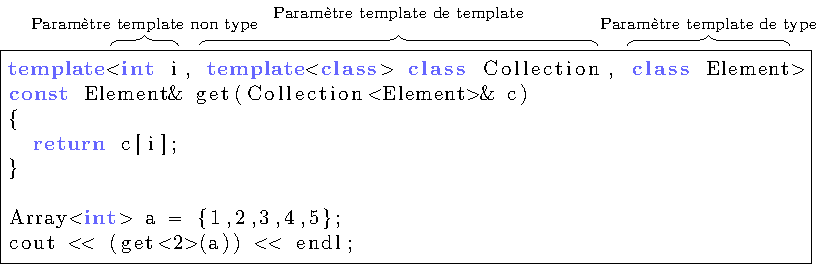
\includegraphics[width=\textwidth]{pics/template.pdf}}
\end{center}
\end{frame}

\begin{frame}
\frametitle{Déduction des arguments templates d'un type}
\begin{itemize}[<+->]
\item Pour déduire les arguments template d'un type, on possède deux informations
	\begin{enumerate}
	\item Le type-id « d'origine » P, combinaison de TTs, de Ts et de Is
	\item Le type-id « sortie » A, sans paramètres template
	\end{enumerate}
\item Le compilateur tente de trouver 
	\begin{itemize}
	\item un template de classe pour TT
	\item un type pour I
	\item une valeur pour I
	\end{itemize}
\item But : obtenir P = A
\end{itemize}
\begin{exampleblock}<+->{Exemple}
	\begin{itemize}
	\item Sur l'exemple précédent, on a
		\begin{itemize}[<+->]
		\item P = \lstinline|int,Collection<Element>|
			\begin{itemize}
			\item TT = \lstinline|Array<int>|, T = \lstinline|int|, I = \lstinline|2|
			\end{itemize}
		\item A = \lstinline|2,Array<int>|
		\end{itemize}		
	\end{itemize}
\end{exampleblock}
\end{frame}

\begin{frame}[containsverbatim]
\frametitle{Exemple}
\begin{itemize}
\item Fichier \texttt{deduct.cpp}
\end{itemize}
\begin{lstlisting}
template<int i, template<class> class Collection, class Element>
Element& get(Collection<Element>& c)
{
	return c[i];
}

template<class E>
class Array
{
	E* a;
	int _size;

	public:
		...
		
		E& operator[](int i) { return a[i]; }
};

int main()
{
	Array<int> a = {1,2,3,4,5};
	cout << (get<2>(a)) << endl;
}
\end{lstlisting}
\end{frame}

\begin{frame}
\frametitle{Déduction d'un type}
\begin{itemize}[<+->]
\item En pratique, A peut être n'importe quel type \cpp
\item P peut être un \texttt{T}, un \texttt{T*}, un \texttt{T\&}, un \texttt{TT<T>}, etc.
	\begin{itemize}
	\item Liste exhaustive pour P : \url{http://en.cppreference.com/w/cpp/language/template_argument_deduction}
	\end{itemize}
\item Sur l'exemple précédent, « à l'évidence », la valeur \texttt{2} ne peut pas être déduite
	\begin{itemize}
	\item Mais \lstinline|Array<int>| le peut
	\end{itemize}
\item La déduction de type est effectuée
	\begin{itemize}
	\item à l'appel d'une fonction
	\item à la prise d'adresse d'une fonction
	\item à l'instanciation explicite d'un template
	\item quand l'inférence de type est utilisée, etc.
	\end{itemize}
\end{itemize}
\end{frame}

\section[Amis]{Templates amis}

\begin{frame}
\frametitle{Amitiés}
\begin{itemize}[<+->]
\item Les déclarations de templates de classe et de fonction peuvent être déclarées amies
\item Si déclaration au sein d'un template de classe, toutes les spécialisations du template sont des amies
	\begin{itemize}
	\item Le seul cas de « transitivité » de la relation d'amitié
	\end{itemize}
\item Les signatures doivent correspondre exactement pour l'amitié
\item Les déclarations d'amitiés ne peuvent référencer des spécialisations partielles
\item Lors de l'amitié d'une spécialisation complète, les arguments par défaut ne peuvent être utilisés
\end{itemize}
\end{frame}

\begin{frame}[containsverbatim]
\frametitle{Exemple}
\begin{itemize}
\item Fichier \texttt{friend-1.cpp}
\end{itemize}
\begin{lstlisting}
template<class T> class B;
template<class T> int add(T t);

class A 
{
	int i;

	public:	
		A(int i) : i(i) {}

	    template<class T>
    	friend class B; // every B<T> is a friend of A
 
    	template<class T>
    	friend int add(T t); // every f<T> is a friend of A
};

template<class T> class B { ... };

template<class T> int add(T t) { ... }
\end{lstlisting}
\end{frame}

\begin{frame}[containsverbatim]
\frametitle{Exemple}
\begin{itemize}
\item Fichier \texttt{friend-2.cpp}
\end{itemize}
\begin{lstlisting}
template<class T> class A {}; // primary
template<class T> class A<T*> {}; // partial
template<> class A<int> {}; // full

class X 
{
    template<class T> friend class A<T*>; // error!
    friend class A<int>; // OK
};

template<class T> void f(int);
template<> void f<int>(int);
 
class Y 
{
    friend void f<int>(int x = 1); // error: default args not allowed
};
\end{lstlisting}
\begin{itemize}
\item Source : cppreference
\end{itemize}
\end{frame}

\begin{frame}[containsverbatim]
\frametitle{Exemple}
\begin{itemize}
\item Fichier \texttt{friend-3.cpp}
\end{itemize}
\begin{lstlisting}
template<class T> // primary
struct A
{
    struct C {}; void f();
    struct D  { void g(); };
};
template<> // full
struct A<int>
{
    struct C {}; int f(); //!= signature
    struct D { void g(); };
};
class B // non-template
{
    template<class T>
    friend struct A<T>::C; // A<int>::C is a friend, as well as all A<T>::C
    template<class T>
    friend void A<T>::f(); // A<int>::f() is not a friend, because the
                           // signatures do not match, but A<char>::f() is
    template<class T>
    friend void A<T>::D::g(); // A<int>::D::g() is not a friend: it is not a member
                              // of A, and A<int>::D is not a specialization of A<T>::D
};
\end{lstlisting}
\begin{itemize}
\item Source : cppreference
\end{itemize}
\end{frame}

\subsection{Amitié et opérateurs}

\begin{frame}
\frametitle{Amitié et opérateurs}
\begin{itemize}[<+->]
\item Utilisation classique d'amitié de template: opérateurs
	\begin{itemize}
	\item P. ex. : injection de flux
	\end{itemize}
\item Deux façons de procéder
	\begin{enumerate}
	\item Opérateur non-template
		\begin{itemize}
		\item Warning
		\end{itemize}
	\item Opérateur template
	\end{enumerate}
\end{itemize}
\begin{block}<+->{Hygiène de programmation}
	\begin{itemize}[<+->]
	\item Utiliser des opérateurs template
		\begin{itemize}
		\item Moins prompt aux erreurs
		\end{itemize}
	\end{itemize}
\end{block}
\end{frame}

\begin{frame}[containsverbatim]
\frametitle{Exemple}
\begin{itemize}
\item Fichier \texttt{friend-op1.cpp}
\end{itemize}
\begin{lstlisting}
template<class T>
class A
{
	T t;
	public:
		A(T t) : t(t) {}
		friend ostream& operator<<(ostream& out, const A& a)
		{
			return out << a.t;
		}
};

int main()
{
	A<int> a(2);
	cout << a << endl;
}
\end{lstlisting}
\end{frame}

\begin{frame}[containsverbatim]
\frametitle{Exemple}
\begin{itemize}
\item Fichier \texttt{friend-op2.cpp}
\end{itemize}
\begin{lstlisting}
template<class T>
class A
{
	T t;
	public:
		A(T t) : t(t) {}

		friend ostream& operator<<(ostream& out, const A& a); //warning
};

template<class T>
ostream& operator<<(ostream& out, const A<T>& a)
{
	return out << a.t;
}

int main()
{
	A<int> a(2);
	cout << a << endl; //error 
}	
\end{lstlisting}
\end{frame}

\begin{frame}[containsverbatim]
\frametitle{Exemple}
\begin{itemize}
\item Fichier \texttt{friend-op3.cpp}
\item Similaire à \texttt{friend-op1.cpp}
\end{itemize}
\begin{lstlisting}
template<class T>
class A
{
	T t;
	public:
		A(T t) : t(t) {}
		
		template<class U>
		friend ostream& operator<<(ostream& out, const A<U>& a);
};

template<class T>
ostream& operator<<(ostream& out, const A<T>& a)
{
	return out << a.t;
}

int main()
{
	A<int> a(2);
	cout << a << endl;
}
\end{lstlisting}
\end{frame}

\begin{frame}[containsverbatim]
\frametitle{Exemple}
\begin{itemize}
\item Fichier \texttt{friend-op4.cpp}
\item Opérateur template
\end{itemize}
\begin{lstlisting}
template<class T> class A; // forward declare to make function declaration possible
template<class T> ostream& operator<<(ostream&, const A<T>&); // declaration
 
template<class T>
class A 
{
	T t;
	public:
	    A(T t) : t(t) {}
    // refers to a full specialization for this particular T 
    friend std::ostream& operator<< <> (std::ostream&, const A&);
};
 
// definition
template<typename T>
ostream& operator<<(ostream& out, const A<T>& a) { return out << a.t; }
 
int main()
{
	A<int> a(2);
	cout << a << endl;
}
\end{lstlisting}
\end{frame}

\begin{frame}[containsverbatim]
\frametitle{Exemple}
\begin{itemize}
\item Fichier \texttt{friend-wtf.cpp}
\end{itemize}
\begin{lstlisting}
template<class T> class A;
template<class T> std::ostream& operator<<(std::ostream&, const A<T>&);
template<class T> A<T> operator+(const T&, const A<T>&);

template<class T>
class A
{
	T i;
	public:
		explicit A(T t) : i(t) {}
		friend A<T> operator+ <>(const T& t, const A<T>& a); //YOU HAVE TO DECLARE THIS HERE
		friend std::ostream& operator<< <>(std::ostream& out, const A<T>& a);		
		A operator +(A<T> a) const { return A(a.i + i); }				
		A operator +(T t) const { return (*this) + A<T>(t); }								
};

template<class T>
std::ostream& operator<<(std::ostream& out, const A<T>& a)
{
	out << a.i; return out;
}

template<class T>
A<T> operator +(const T& t, const A<T>& a) { return A<T>(t) + a; }
\end{lstlisting}
\end{frame}

\section{Templates variadiques}

\begin{frame}
\frametitle{Les arguments variables en nombre}
\begin{itemize}[<+->]
\item Jusqu'à présent, en \cpp, on n'a pas vu de manière «~satisfaisante~» comment passer un nombre d'arguments variables en nombre
	\begin{itemize}
	\item Comme en \texttt{C}~: utiliser \texttt{va\_list}
	\item \texttt{std::initializer\_list}
	\end{itemize}
\item Grâce aux templates, on peut faire mieux
\item Templates variadiques
\item Syntaxe : \lstinline|template<class Args> A f(Args ... args)|
	\begin{itemize}
	\item Pour des templates de classe, les arguments variadiques doivent être les derniers
	\item Pour des templates de fonction, les paramètres explicites doivent être les derniers
	\end{itemize}
\item Autre utilité : certains templates ont des paramètres «~cachés~»
\begin{itemize}
	\item \texttt{map}, \texttt{vector}, \texttt{list}, etc.
	\item On ne pouvait pas les utiliser avec \texttt{get} (Slide 24, 26)
	\item Erreur de substitution
\end{itemize}
\end{itemize}
\end{frame}

\begin{frame}[containsverbatim]
\frametitle{Exemple}
\begin{lstlisting}
template<class ... Types> struct Tuple {};
Tuple<> t0;           // Types contains no arguments
Tuple<int> t1;        // Types contains one argument: int
Tuple<int, float> t2; // Types contains two arguments: int and float
Tuple<0> error;       // 0 is not a type
\end{lstlisting}
\begin{lstlisting}
template<class ... Types> void f(Types ... args);
f();       // OK: args contains no arguments
f(1);      // OK: args contains one argument: int
f(2, 1.0); // OK: args contains two arguments: int and double
\end{lstlisting}
\begin{lstlisting}
template<typename... Ts, typename U> struct Invalid; // Error: Ts.. not at the end
 
template<typename ...Ts, typename U, typename=void>
void valid(U, Ts...);     // OK: can deduce U
//void valid(Ts..., U);   // error : cannot deduce
 
valid(1.0, 1, 2, 3);      // OK: deduces U as double, Ts as {int,int,int}
\end{lstlisting}
\end{frame}

\begin{frame}
\frametitle{Extension de pack}
\begin{itemize}[<+->]
\item Terminologie : \texttt{Args ... args} est un pack de paramètres
\item On accède aux paramètres un par un en « étendant » le pack
	\begin{itemize}
	\item \texttt{args...} est l'expansion de pack
	\end{itemize}
\item L'expansion est effectuée récursivement, paramètre par paramètre
\item On peut «~préfixer~» l'extension
	\begin{itemize}
	\item Exemple : \texttt{\&args...}
	\end{itemize}
\item Si packs sont imbriqués ou étendus « ensemble », les règles sont assez complexes
%\item Utilité de \texttt{std::forward}
\end{itemize}
\end{frame}

\begin{frame}[containsverbatim]
\frametitle{Exemple}
\begin{itemize}
\item Fichier \texttt{variadic.cpp}
\end{itemize}
\begin{lstlisting}
template<typename T>
T sum(T v) 
{
  return v;
}

template<class T, class ... Args>
T sum(T first, Args... args) 
{
  return first + sum(args...);
}

int main()
{
	int s = sum(1,2,3,4);
	cout << s << endl;

	string s1 = "a", s2 = "b", s3 = "c", s4 = "d";
	string str = sum(s1, s2, s3, s4);
	cout << str << endl;		
}
\end{lstlisting}
\end{frame}

\begin{frame}
\frametitle{Le problème de forwarding}
\begin{itemize}[<+->]
\item Une fonction \lstinline|void f(int& i, int& j, int& k)| ne peut pas être appelée avec des immédiats
	\begin{itemize}
	\item Ni aucune rvalue
	\end{itemize}
\item On ne peut pas convertir implicitement une rvalue en rvalue
\item « Solution » : \lstinline|void f(const int& i, const int& j, const int& k)|
\item Inconvénient : on ne peut plus modifier les paramètres
	\begin{itemize}
	\item Et c'est une bonne chose si on passe des immédiats
	\end{itemize}
\item Si on veut en modifier certains, il ne faut mettre que certains \lstinline|const|
\item Sur un template variadique, c'est probablement voulu
	\begin{itemize}
	\item Par exemple, si on veut écrire une fonction qui prend en paramètre une fonction $f$, et ses arguments
	\item \scriptsize{\lstinline|auto call_function(Function f, Args& ... args)|}
	\end{itemize}
\end{itemize}
\end{frame}

\begin{frame}[containsverbatim]
\frametitle{Ce que l'on ne veut pas faire}
\begin{itemize}
\item Écrire toutes les combinaisons de const et pas const
\end{itemize}
\begin{lstlisting}
template <class A, class B, class C>
void f(A& a, B& b, C& c);

template <class A, class B, class C>
void f(const A& a, B& b, C& c);

template <class A, class B, class C>
void f(A& a, const B& b, C& c);

template <class A, class B, class C>
void f(A& a, B& b, const C& c);

template <class A, class B, class C>
void f(const A& a, const B& b, C& c);

template <class A, class B, class C>
void f(const A& a, B& b, const C& c);

template <class A, class B, class C>
void f(A& a, const B& b, const C& c);

template <class A, class B, class C>
void f(const A& a, const B& b, const C& c);
\end{lstlisting}
\begin{itemize}
\item Avec des templates variadiques, c'est impossible
\end{itemize}
\end{frame}

\begin{frame}[containsverbatim]
\frametitle{Astuce : utiliser les références de rvalue}
\begin{lstlisting}
template<class Function, class ... Args>
auto call_function(Function f, Args&& ... args) -> decltype(f(args...))
{
	return f(args...);
}

void print(int i) {  cout << i << endl; }

void increment(int & i) { i++; }

int main()
{
	call_function(print, 2);

	int i = 3;
	call_function(increment, i);
	print(i);

	call_function(increment, 3); //wtf ?!
}
\end{lstlisting}
\begin{itemize}
\item Problème : on ne veut pas que \lstinline|call_function(increment, 3)| compile
\end{itemize}
\end{frame}

\begin{frame}[containsverbatim]
\frametitle{Solution}
\begin{itemize}
\item Fichier \texttt{fwd.cpp}
\end{itemize}
\begin{lstlisting}
template<class Function, class ... Args>
auto call_function(Function f, Args&& ... args) -> decltype(f(args...))
{
	return f(forward<Args>(args)...);
}

void print(int i) {  cout << i << endl; }

void increment(int & i) { i++; }

int main()
{
	call_function(print, 2);

	int i = 3;
	call_function(increment, i);
	print(i);

	//call_function(increment, 3); //doesn't compile anymore
}
\end{lstlisting}
\end{frame}

\begin{frame}
\frametitle{Fonctionnement}
\begin{itemize}[<+->]
\item Rappel : \texttt{\&\&} crée des références de lvalue
\item \texttt{std::forward<T>(T \&\& t)} est résolu en
	\begin{itemize}
	\item \texttt{T\&} si \texttt{t} est une référence de rvalue
	\item \texttt{std::move} sinon
	\end{itemize}
\item Le risque de « modification d'immédiat » est éliminé par \texttt{std::move}
\item Sucre syntaxique pour \lstinline|static_cast<T&&>(t)|
\end{itemize}
\end{frame}

\begin{frame}[containsverbatim]
\frametitle{Différence entre \texttt{move} et \texttt{forward}}
\begin{itemize}
\item Fichier \texttt{move-fwd.cpp}
\end{itemize}
\begin{lstlisting}
void overloaded(const int & arg )  {  cout << "by lvalue\n";  }

void overloaded(int && arg ) {  cout << "by rvalue\n";  }
     
template<class T>
void forwarding( T && arg ) 
{
	cout << "by simple passing: "; overloaded(arg);
	cout << "via std::forward: "; overloaded( forward<T>(arg) );
	cout << "via std::move: "; overloaded( move(arg) ); //arg is now invalidated	
}

int main() 
{
	cout << "initial caller passes rvalue:\n";
	forwarding(5);
	cout << endl;

	cout << "initial caller passes lvalue:\n";
	int x = 5;
	forwarding(x);
}
\end{lstlisting}
\end{frame}

\section[Spécialisation]{Spécialisation de templates}

\begin{frame}
\frametitle{Overview}
\begin{itemize}[<+->]
\item La plupart du temps, on écrit une classe template et elle est «~valide~» pour tous les types
	\begin{itemize}
	\item Parfois, on veut particulariser la classe pour certains types
	\end{itemize}
\item Deux types de spécialisation
	\begin{enumerate}
	\item \emph{complète} : tous les arguments templates sont fixés
	\item \emph{partielle} : certains arguments templates sont spécialisés
	\end{enumerate}
\item Permet de personnaliser le comportement pour certains arguments template
	\begin{itemize}
	\item Efficacité
	\end{itemize}
\end{itemize}
\begin{exampleblock}<+->{Exemple}
	\begin{itemize}[<+->]
	\item \texttt{vector} est complètement spécialisé pour les vecteurs booléens
	\item Économie de taille
	\end{itemize}
\end{exampleblock}
\end{frame}

%\subsection{Spécialisation complète de templates}

\begin{frame}
\frametitle{Spécialisation complète de templates}
\begin{itemize}[<+->]
\item Parfois, on veut spécialiser l'implémentation d'un template pour certains types
	\begin{itemize}
	\item Efficacité
	\item Fonctionnalité
	\end{itemize}
\item Possibilité de fournir de nouvelles fonctionnalités
	\begin{itemize}
	\item ... voire de changer complètement l'interface publique
	\end{itemize}
\item Divergence possible grâce à l'instanciation
	\begin{itemize}
	\item Code « généré », \lstinline|vector<int>| est un type complet, et différent de \lstinline|vector<bool>|
	\end{itemize}
\end{itemize}
\begin{block}<+->{Hygiène de programmation}
	\begin{itemize}
	\item Éviter les ambiguïtés et le code obscur
	\end{itemize}
\end{block}
\end{frame}

\begin{frame}[containsverbatim]
\frametitle{Exemple}
\begin{itemize}
\item Fichier \texttt{full.cpp}
\end{itemize}
\begin{lstlisting}
struct R {};
struct S { S() { cout << "+S" << endl; } };

template<class T> struct A
{
	int i; T t;
	A(int i, T t) : i(i), t(t) { cout << "+A<T>" << endl; }			
};

template<> struct A<bool>
{
	S s; bool b;
	A(bool b) : b(b), s(S()) { cout << "+A<bool>" << endl; }
};

int main()
{
	A<R> a(2,R());
	cout << a.i << endl;	
	A<bool> b(true);
	//cout << b.i << endl; //error : no A<bool>::i
	cout << b.b << endl;
}
\end{lstlisting}
\end{frame}

\begin{frame}
\frametitle{Spécialisation partielle de templates}
\begin{itemize}[<+->]
\item La spécialisation complète de templates ne permet plus de paramétrisation « générique » du template
	\begin{itemize}
	\item On a spécifié que \lstinline|vector<bool>| se comporte particulièrement
	\item On ne sait pas dire « un vecteur de pointeurs se comporte différemment »
	\end{itemize}
\item La spécialisation partielle de templates permet d'effectuer cela
\end{itemize}
\begin{exampleblock}<+->{Exemple}
	\begin{itemize}[<+->]
	\item \lstinline|class A<T,U>| : template primaire
	\item \lstinline|class A<T*,U>| : spécialisation partielle où le premier argument est un pointeur
	\item \lstinline|class A<T,T>| : spécialisation partielle où les deux arguments sont identiques
	\end{itemize}
\end{exampleblock}
\end{frame}

\begin{frame}[containsverbatim]
\frametitle{Exemple}
\begin{itemize}
\item Fichier \texttt{partial-1.cpp}
\end{itemize}
\begin{lstlisting}
template<class T> struct A
{	
	T t;
	A(T t) : t(t) {}
	
	void print() { cout << t << endl; }
};

template<class T> struct A<T*>
{
	T* t;
	A(T* t) : t(t) {}
	
	void print() { cout << *t << endl; }
};

int main()
{
	int i = 2;
	A<int> a1(i); a1.print();
	A<int*> a2(&i); a2.print();
}
\end{lstlisting}
\end{frame}

\begin{frame}
\frametitle{Ordre partiel}
\begin{itemize}[<+->]
\item Quand un template de classe est instancié, il peut exister plusieurs spécialisations partielles
\item Le compilateur doit décider s'il utilise le template primaire ou une spécialisation
\end{itemize}
\begin{exampleblock}<+->{Règle}
	\begin{enumerate}[<+->]
	\item Correspondance exacte 
		\begin{itemize}
		\item Les arguments template correspondent : utilisation de la spécialisation
		\end{itemize}
	\item Si plus d'une spécialisation correspond, « la plus spécialisée » est utilisée
		\begin{itemize}
		\item Si aucune n'est plus spécialisée : erreur (ambiguïté)
		\end{itemize}
	\item Template primaire
	\end{enumerate}
\end{exampleblock}
\end{frame}

\begin{frame}[containsverbatim]
\frametitle{Illustration}
\begin{itemize}
\item Fichier \texttt{partial-2.cpp}
\end{itemize}
\begin{lstlisting}
template<class T1, class T2, int I>
class A {}; // primary template
 
template<class T, int I>
class A<T, T*, I> {}; // partial specialization where T2 is a pointer to T1
 
template<class T, class T2, int I>
class A<T*, T2, I> {}; // partial specialization where T1 is a pointer
 
template<class T>
class A<int, T*, 5> {}; // partial specialization where T1 is int, I is 5,
                        // and T2 is a pointer 
template<class X, class T, int I>
class A<X, T*, I> {}; // partial specialization where T2 is a pointer

int main()
{
	A<int, int, 1> a1;   // no specializations match, uses primary template
	A<int, int*, 1> a2;  // uses partial specialization #1 (T=int, I=1)
	A<int, char*, 5> a3; // uses partial specialization #3, (T=char)
	A<int, char*, 1> a4; // uses partial specialization #4, (X=int, T=char, I=1)
	//A<int*, int*, 2> a5; // error: matches #2 (T=int, T2=int*, I=2)
                     	   //        matches #4 (X=int*, T=int, I=2)
                           // neither one is more specialized than the other
}
\end{lstlisting}
\end{frame}

\begin{frame}[containsverbatim]
\frametitle{Exemple}
\begin{itemize}
\item On voudrait spécialiser \texttt{Array<T,N>} pour que
	\begin{enumerate}
	\item si utilisé avec une adresse, on imprime les éléments déférencés
	\item Si utilisé « comme un tableau 2D », qu'on l'affiche sous forme matricielle
	\end{enumerate}
\item Il faut spécialiser le template dans \texttt{array.hpp}
\end{itemize}
\begin{lstlisting}
Array<int*,3> a_add;
int n[3];
for(unsigned i = 0; i < 3; i++)
{
	n[i] = i + 1;
    a_add[i] = &(n[i]);
}
cout << a_add << endl; //objective : 1 2 3
\end{lstlisting}
\begin{lstlisting}
Array<Array<int,2>,3> a2d = {{1,2},{3,4},{5,6}};
cout << a2d << endl; //objective : 1 2
                     //            3 4
                     //            5 6
\end{lstlisting}
\end{frame}

\begin{frame}[containsverbatim]
\frametitle{Solution : premier cas}
\begin{itemize}
\item Fichier \texttt{array-spec.hpp}
\end{itemize}
\begin{lstlisting}
template<class T, int N> class Array<T*,N>
{
	T ** t;       
    
	public:
		Array() : t(new T*[N]) 
        {
            for(int i = 0; i < N; i++)
                t[i] = nullptr;
        }
        
    ...
    
};

template<class T, int N>
std::ostream& operator<<(std::ostream& out, const Array<T*,N>& a)
{
    out << "{ ";
    for(unsigned i = 0; i < a.size() - 1; i++)
        out << *(a[i]) << " , ";
    out << *(a[a.size() - 1]) << " }";

    return out;
}
\end{lstlisting}
\end{frame}

\begin{frame}[containsverbatim]
\frametitle{Solution : second cas}
\begin{itemize}
\item Fichier \texttt{array-spec.hpp}
\end{itemize}
\begin{lstlisting}
template<class T, int N, int M> class Array<Array<T,M>, N>
{
	Array<T,M> * t;       
    
	public:
		Array() : t(new Array<T,M>[N]) {}
		
	...
};

template<class T, int N, int M>
std::ostream& operator<<(std::ostream& out, const Array<Array<T,M>,N>& a)
{
    for(unsigned i = 0; i < N; i++)
    {
        for(unsigned j = 0; j < M; j++)
            out << a[i][j] << " ";    
        out << std::endl;
    }

    return out;
}
\end{lstlisting}
\end{frame}

\begin{frame}
\frametitle{Debriefing}
\begin{itemize}[<+->]
\item Ça fonctionne
\end{itemize}
\begin{alertblock}<+->{Problème}
	\begin{itemize}[<+->]
	\item Il y a énormément de copier / coller
	\end{itemize}
\end{alertblock}
\begin{block}<+->{Solution}
	\begin{itemize}[<+->]
	\item Utiliser SFINAE
		\begin{itemize}
		\item En dur, avec \texttt{std::enable\_if} ou avec les concepts
		\item Cf. Ch. 14
		\end{itemize}
	\end{itemize}
\end{block}
\end{frame}

\end{document}